\documentclass{article}

\usepackage{microtype}
\usepackage{graphicx}
\usepackage{booktabs}
\usepackage{amsmath}
\usepackage{amssymb}
\usepackage{tikz}
\usepackage{algorithm}
\usepackage{algorithmic}
\usepackage{hyperref}

\usepackage{mlsys2025}
\renewcommand{\ttdefault}{cmtt}

\mlsystitlerunning{Structured Exact-Budget Mixed Precision for Task-Aware LLM Quantization}

\definecolor{taqgreen}{HTML}{0F7F64}
\definecolor{taqblue}{HTML}{315F85}
\definecolor{taqclay}{HTML}{C8643D}
\definecolor{taqgold}{HTML}{D4A72C}
\definecolor{taqgray}{HTML}{EEF0EA}

\newcommand{\method}{TA-MPQ}
\newcommand{\policyid}{\texttt{gpf\_refine\_00\_i0112}}
\newcommand{\hashshort}{\texttt{7caae6e...2043e4}}

\begin{document}

\twocolumn[
\mlsystitle{Structured Exact-Budget Mixed Precision for Task-Aware LLM Quantization}

\begin{mlsysauthorlist}
\mlsysauthor{Anonymous Authors}{anon}
\end{mlsysauthorlist}
\mlsysaffiliation{anon}{Anonymous Institution}
\mlsyscorrespondingauthor{Anonymous Authors}{anonymous@example.com}

\mlsyskeywords{post-training quantization, mixed precision, large language models, code generation, systems}

\vskip 0.3in

\begin{abstract}
Mixed-precision quantization can in principle allocate high precision only where it matters for a target workload, but unconstrained search can be unstable when every promotion must be balanced against a deployment budget. We study this issue in a task-aware mixed-precision quantization pipeline for Qwen3.5-9B, initially targeting coding and math workloads. Our main engineering finding is that evolutionary crossover is a poor fit for an exact footprint constraint: crossover explores policies, while budget repair subsequently rewrites them. We replace it with a deterministic frontier search that starts from a uniform INT4 anchor, promotes high-value groups to INT8, demotes lower-value groups to INT2, and keeps the raw weight footprint matched to uniform INT4. The resulting 2/4/8-bit policies have estimated average bit-widths near 4 bits. Empirically, the coding policy matches uniform INT4 on MMLU-coding last100 (91\%) but improves over uniform INT4 on HumanEval base (84.8\% vs. 81.1\%) and HumanEval+ (79.9\% vs. 76.8\%). On BigCodeBench-Hard, it reaches 23.65\% pass@1 versus 16.89\% for uniform INT4, recovering 10 of the 18 tasks lost by INT4 relative to BF16. A MATH-oriented exact-budget policy similarly improves MATH-500 last100 from 80\% to 84\%, near the BF16 score of 86\%. These results support a narrower but more defensible claim: structured exact-budget mixed precision is a reproducible mainline that recovers part of the INT4 degradation on target workloads.
\end{abstract}
]

\printAffiliationsAndNotice{}

\section{Introduction}

Large language model (LLM) deployment is increasingly governed by memory footprint, throughput, and hardware availability rather than only by model quality. Post-training quantization (PTQ) is attractive because it compresses an existing model without full retraining, and recent work has shown that 8-bit and 4-bit quantization can preserve much of the performance of large transformer models \cite{dettmers2022llm,frantar2023gptq,xiao2023smoothquant,lin2024awq}. However, uniform quantization applies the same precision everywhere. This ignores the fact that different layers, projections, and tasks may have different precision requirements.

Mixed-precision quantization (MPQ) attempts to exploit this non-uniformity. A task-aware MPQ system asks a simple question: given a target task and a fixed memory budget, which groups of weights should receive more bits, and where can the system safely spend fewer bits? This question becomes difficult once the budget is strict. Promoting a group from 4-bit to 8-bit is only useful if the policy can pay for that promotion by demoting other groups or by using slack elsewhere. A search algorithm that proposes policies without respecting this coupling can waste most of its effort exploring infeasible or heavily repaired candidates.

This paper reports the current state of \method{}, a task-aware MPQ pipeline for Qwen3.5-9B \cite{qwen2025model}. The project originally used evolutionary search over quantization policies. That route was appealing because it could search a large combinatorial space and incorporate surrogate feedback. In practice, it was hard to make rigorous progress. Crossover combined parent policies without regard to the exact footprint target; budget repair then modified the child, often erasing the intended structure of the crossover. Surrogate models were also data-limited, making their ranking uncertain when only a small number of real PTQ candidates had been evaluated.

We therefore changed the mainline. Instead of asking an evolutionary algorithm to discover a policy from scratch, we build a deterministic frontier from a uniform INT4 anchor. Each step along the frontier is an interpretable trade: promote high-value groups to 8-bit and offset the extra cost with 2-bit demotions on lower-value groups. The target budget is the raw weight footprint of a uniform INT4 model. This gives us an exact-budget policy family, a clear search coordinate, and a practical way to debug which groups receive which precision.

Our current best policy, \policyid{}, is a real quantized model artifact produced through a source PTQ path using LLM Compressor tooling \cite{llmcompressor}. It uses the bit space $\{2,4,8\}$ over 249 per-block component groups. It assigns 57 groups to 2-bit, 80 groups to 4-bit, and 112 groups to 8-bit. By parameter mass, this corresponds to 26.00\% at 2-bit, 61.02\% at 4-bit, and 12.98\% at 8-bit. The estimated average bit-width is 3.9989, and the raw weight footprint is 3.694 GB, matching the INT4 target with only 0.026\% slack.

The empirical story is deliberately conservative. On MMLU-coding last100 \cite{hendrycks2021mmlu}, the coding mixed policy reaches 91\%, matching uniform INT4 but not exceeding it. On HumanEval and EvalPlus \cite{chen2021humaneval,liu2023evalplus}, it recovers a meaningful portion of the INT4 degradation: HumanEval base improves from 81.1\% to 84.8\%, and HumanEval+ improves from 76.8\% to 79.9\%. On BigCodeBench-Hard \cite{zhuo2024bigcodebench}, it improves over uniform INT4 from 25/148 to 35/148 passing tasks. On MATH-500 last100 \cite{hendrycks2021math}, a MATH-oriented exact-budget policy improves over uniform INT4 from 80/100 to 84/100, while BF16 reaches 86/100.

Our contributions are as follows:
\begin{itemize}
    \item We identify a practical failure mode of evolutionary MPQ under exact budget constraints: crossover and budget repair are structurally misaligned.
    \item We introduce a deterministic exact-budget frontier for 2/4/8-bit task-aware quantization, anchored at uniform INT4.
    \item We report a reproducible Qwen3.5-9B mixed policy with explicit bit distribution, budget accounting, and real PTQ artifacts.
    \item We provide a current evaluation snapshot on MMLU-coding, HumanEval/EvalPlus, and BigCodeBench-Hard execution, emphasizing both positive results and limitations.
\end{itemize}

\section{Related Work}

\paragraph{Post-training quantization for LLMs.}
LLM quantization has progressed from weight-only compression to activation-aware and outlier-aware techniques. LLM.int8() showed that careful handling of activation outliers can make 8-bit inference practical for large transformer models \cite{dettmers2022llm}. GPTQ introduced a second-order weight-only post-training quantization method that can compress large models to low precision with limited calibration data \cite{frantar2023gptq}. SmoothQuant shifts quantization difficulty from activations to weights by smoothing activation outliers \cite{xiao2023smoothquant}, while AWQ preserves salient weights based on activation-aware importance estimates \cite{lin2024awq}. These methods motivate the empirical premise behind \method{}: uniform 8-bit is often close to BF16, while uniform 4-bit may lose measurable accuracy on harder tasks. Our focus is not a new quantizer kernel, but a policy-search layer above PTQ that decides where different bit-widths should be assigned.

\paragraph{Mixed precision as allocation.}
Mixed precision reframes quantization as a resource-allocation problem. Instead of asking whether a whole model should be 4-bit or 8-bit, it asks which submodules deserve extra precision under a budget. This is a natural fit for transformer models because attention projections, MLP projections, and output heads are not equally important for every workload. The challenge is that MPQ search spaces are combinatorial and deployment budgets are discrete. A method that ignores the coupling between high-precision promotions and low-precision compensation can produce candidates that look plausible before repair but become quite different after repair. The exact-budget frontier in this paper is a deliberately constrained response to that issue.

\paragraph{Evaluation for code generation.}
Coding benchmarks differ substantially in how they expose quantization error. Multiple-choice coding tasks such as MMLU-coding measure recognition and selection. HumanEval evaluates function synthesis against unit tests \cite{chen2021humaneval}; EvalPlus strengthens HumanEval with additional tests that catch under-specified or brittle solutions \cite{liu2023evalplus}. BigCodeBench expands the setting to more realistic programming tasks with dependencies, larger prompts, and richer execution requirements \cite{zhuo2024bigcodebench}. This distinction matters for our current results: MMLU-coding does not separate mixed from uniform INT4, while HumanEval/EvalPlus and BigCodeBench-Hard both show a mixed advantage over uniform INT4.

\paragraph{Positioning.}
The present work is best understood as a systems paper about experimental control. It does not claim that the current sensitivity profiler is optimal, nor that the chosen policy is globally optimal. Instead, it argues that the policy-search coordinate matters. A deterministic exact-budget frontier gives a stable object to measure, reproduce, and debug. This is a prerequisite for credible claims about task-aware MPQ, especially when benchmark differences can be only a few percentage points.

\section{Problem Setting}

Let a pretrained model be partitioned into $G$ quantization groups. In our implementation, groups correspond to per-block components such as attention projections, linear attention projections, MLP up/gate/down projections, and the language modeling head. Each group $g \in \{1,\dots,G\}$ has a parameter count $n_g$ and receives a bit-width $b_g$ from a discrete set $\mathcal{B}$. For the current route, $\mathcal{B}=\{2,4,8\}$.

We define the raw weight budget of a policy $p$ as
\begin{equation}
B(p) = \sum_{g=1}^{G} n_g b_g.
\end{equation}
The target budget is the raw footprint of a uniform INT4 policy:
\begin{equation}
B_{\text{INT4}} = \sum_{g=1}^{G} 4n_g.
\end{equation}
The search objective is not simply to maximize the number of 8-bit groups. It is to choose bit-widths that improve task performance while satisfying $B(p) \le B_{\text{INT4}}$ up to negligible slack. This is why 8-bit promotions require compensating 2-bit demotions: promoting group $g$ from 4-bit to 8-bit costs $4n_g$ extra bits, while demoting group $h$ from 4-bit to 2-bit saves $2n_h$ bits.

The task-aware part enters through a ranking signal. For a target task, we estimate which groups are likely to benefit from higher precision and which groups are likely to tolerate lower precision. In the current experiments, the ranking signal is derived from MMLU-coding development prompts. The final policy is selected by coarse-to-fine evaluation along a structured frontier, not by random mutation or crossover.

\paragraph{Design requirements.}
The current route is guided by three practical requirements. First, every candidate should have a transparent raw footprint so that comparisons against uniform INT4 are not ambiguous. Second, a candidate should be easy to inspect at the group level; otherwise a surprising result cannot be traced back to concrete precision assignments. Third, the search procedure should spend most evaluations on policies that are already near the deployment budget, rather than relying on a large repair step after sampling. These requirements intentionally bias the method toward structured local optimality rather than unconstrained global exploration.

\section{Why We Replaced Evolutionary Search}

The previous pipeline used a loop of candidate generation, surrogate prediction, search, PTQ execution, and evaluation. This is a natural framework for MPQ when real evaluations are expensive. However, it exposed three issues.

\paragraph{Crossover conflicts with exact budget.}
Evolutionary crossover combines assignments from two parent policies. The child may inherit expensive 8-bit assignments from both parents without inheriting the exact compensating demotions. A repair step must then bring the policy back under budget. This repair is not a small implementation detail: under a tight INT4-sized target, it can change a large fraction of the child policy. The resulting candidate is no longer a clean semantic combination of the parents.

\paragraph{Surrogate ranking was underdetermined.}
The surrogate route depends on real evaluated policies. Early datasets were too small relative to the feature dimension, and ranking confidence was limited. This matters because a few points of accuracy on small task slices can be sampling noise. A weak surrogate can help propose candidates, but it should not dominate when the target metric is noisy.

\paragraph{The search space needed a better coordinate.}
The most actionable variable was not a general genome over all bit assignments. It was the amount and placement of INT8 under an INT4-sized budget. Once this became clear, a frontier parameterization was more appropriate than unconstrained random search.

The structured route therefore gives up some global exploration in exchange for interpretability and budget stability. It is easier to ask why a group was promoted, why another was demoted, and how far along the frontier a candidate lies.

\section{Structured Exact-Budget Frontier}

Algorithm~\ref{alg:frontier} summarizes the current policy construction. The search starts from uniform INT4 and iteratively considers promotions and demotions. Candidate promotions are ranked by the estimated task value of moving from 4-bit to 8-bit. Candidate demotions are ranked by the estimated cost of moving from 4-bit to 2-bit. The frontier builder then adds 8-bit promotions while selecting enough low-cost demotions to maintain the budget.

\begin{algorithm}[t]
\caption{Exact-budget 2/4/8 frontier construction}
\label{alg:frontier}
\begin{algorithmic}[1]
\STATE \textbf{Input:} groups $g=1,\dots,G$, parameter counts $n_g$, promotion scores $s^+_g$, demotion costs $s^-_g$, target budget $B_{\text{INT4}}$
\STATE Initialize all groups to 4-bit: $b_g \leftarrow 4$
\STATE Sort candidate promotions by descending $s^+_g$
\STATE Sort candidate demotions by ascending $s^-_g$
\STATE Initialize frontier $\mathcal{F} \leftarrow \{b\}$
\FOR{promotion $g$ in ranked promotions}
    \STATE Tentatively set $b_g \leftarrow 8$
    \WHILE{$B(b) > B_{\text{INT4}}$}
        \STATE Select next available low-cost demotion $h$
        \STATE Set $b_h \leftarrow 2$
    \ENDWHILE
    \STATE Append repaired policy $b$ to frontier $\mathcal{F}$
\ENDFOR
\STATE Coarsely evaluate snapshots from $\mathcal{F}$; refine near the best region
\STATE \textbf{Return} selected policy
\end{algorithmic}
\end{algorithm}

\paragraph{Grouping.}
The current policy uses \texttt{per\_block\_component} grouping, producing 249 groups. This is a compromise between layer-level grouping, which is too coarse, and tensor-level grouping, which makes search and reporting harder. Per-block components map naturally to transformer structure and give us interpretable units such as \texttt{block:11:self\_attn.k\_proj} or \texttt{block:22:mlp.down\_proj}.

\paragraph{Candidate selection.}
The frontier is sampled coarsely to identify promising regions, then resampled locally. The selected policy is \policyid{} with hash \hashshort{}. It was selected from path index 112 and then quantized into a real artifact. Selection used MMLU-coding development slices; final reported results include held-out last100 and transfer evaluation.

\paragraph{Budget accounting.}
All budget claims in this paper are raw weight footprint claims. We do not claim that raw footprint equality implies equal peak VRAM, equal kernel dispatch overhead, or equal tokens/sec. Mixed precision can introduce kernel and dequantization overhead. End-to-end memory and throughput should be measured separately.

\paragraph{Coarse-to-fine search.}
The frontier is not evaluated exhaustively. The practical workflow is to sample the ordered path at coarse intervals, identify a region where validation accuracy is strongest, and then subdivide that region. This converts a high-dimensional mixed-precision problem into a one-dimensional ordered search over progressively more aggressive 8-bit promotion and 2-bit compensation. The important property is that each candidate on the path is interpretable: moving forward generally means spending more 8-bit precision on groups ranked as valuable while accepting more 2-bit demotion elsewhere.

\paragraph{Why 2-bit is included.}
The exact INT4-sized target makes 8-bit promotions expensive. If the search space were only $\{4,8\}$, any nontrivial 8-bit allocation would exceed the raw INT4 footprint. Including 2-bit groups provides a budget-balancing mechanism. This does not mean the method is trying to make the model mostly 2-bit. In the selected policy, only 26.00\% of parameter mass is 2-bit and only 12.98\% is 8-bit; most parameter mass remains 4-bit. The 2-bit assignments are therefore best viewed as targeted compensation for high-value 8-bit promotions.

\paragraph{Failure modes we can now diagnose.}
The structured route makes several failure cases explicit. If mixed matches INT4 on a task, as it currently does on MMLU-coding, then either the task does not expose the precision allocation benefit, the ranking signal is not aligned with that task, or the INT4 baseline is already strong enough that the margin is hidden by evaluation noise. If mixed improves on generative tasks, as it currently does on HumanEval/EvalPlus, then the next question is whether the same pattern holds on larger and more realistic code-generation benchmarks. This diagnostic clarity was harder to obtain under the old evolutionary route because candidate semantics were blurred by crossover and repair.

\section{Experimental Setup}

\paragraph{Model and baselines.}
All experiments use Qwen3.5-9B. We compare four model variants:
\begin{enumerate}
    \item BF16 native model.
    \item Uniform INT8 quantized model.
    \item Uniform INT4 quantized model.
    \item Mixed 2/4/8-bit \method{} policy at the raw INT4 budget.
\end{enumerate}
The uniform INT4 baseline is the primary size baseline. Uniform INT8 is a strong quality baseline and often remains close to BF16. The mixed policy aims to recover INT4 degradation without increasing the raw weight footprint.

\paragraph{Tasks.}
We evaluate multiple coding-oriented workloads and one math workload. MMLU-coding is a multiple-choice coding subset evaluated with a simple-evals style prompt and a 4096-token generation wall. HumanEval and HumanEval+ use the official EvalPlus evaluator with greedy generation and a 768-token wall. BigCodeBench-Hard uses the official BigCodeBench instruct prompt builder and official execution evaluator. MATH-500 last100 uses a simple-evals non-thinking prompt with greedy generation and a 4096-token wall.

\paragraph{Metrics.}
For MMLU-coding and MATH-500 we report accuracy, length-capped counts, and latency. For HumanEval/EvalPlus we report pass@1 on base and plus tests. For BigCodeBench-Hard we report pass@1, pass counts, capped generations, and completion-token statistics. All current results are single-run snapshots and should be interpreted as engineering evidence rather than final statistical claims.

\paragraph{Prompt and token-wall controls.}
Prompt choice materially changed early results in this project. We therefore moved coding multiple-choice evaluation to a simple-evals style prompt and raised the MMLU-coding generation wall to 4096 tokens. For HumanEval/EvalPlus, we keep the official EvalPlus generation setting of 768 max new tokens because the task is function completion rather than long-form reasoning. For BigCodeBench, we use the official prompt builder and record length-capped completions separately from execution pass rates. A capped generation is treated as a protocol warning because the model may have been truncated before producing a valid final answer.

\paragraph{Artifact hygiene.}
Each quantized policy is materialized as a real artifact before benchmark evaluation. For BigCodeBench, generation and execution are separated: samples are checkpointed to persistent storage as they are produced, and execution grading is run afterward. This design is intentionally conservative. Execution environments for code benchmarks can fail for reasons unrelated to model quality, such as missing dependencies or sandbox timeouts. Persisting generations first prevents evaluator instability from destroying the primary model outputs and allows re-grading without regenerating model completions.

\begin{figure}[t]
\centering
\resizebox{\columnwidth}{!}{%
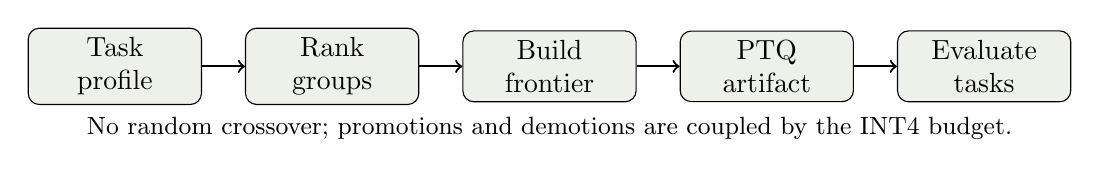
\begin{tikzpicture}[x=0.92cm,y=0.72cm]
  \node[draw,rounded corners,fill=taqgray,align=center,minimum width=2.2cm,minimum height=0.75cm] (p) at (0,0) {Task\\profile};
  \node[draw,rounded corners,fill=taqgray,align=center,minimum width=2.2cm,minimum height=0.75cm] (r) at (3,0) {Rank\\groups};
  \node[draw,rounded corners,fill=taqgray,align=center,minimum width=2.2cm,minimum height=0.75cm] (f) at (6,0) {Build\\frontier};
  \node[draw,rounded corners,fill=taqgray,align=center,minimum width=2.2cm,minimum height=0.75cm] (q) at (9,0) {PTQ\\artifact};
  \node[draw,rounded corners,fill=taqgray,align=center,minimum width=2.2cm,minimum height=0.75cm] (e) at (12,0) {Evaluate\\tasks};
  \draw[->,thick] (p) -- (r);
  \draw[->,thick] (r) -- (f);
  \draw[->,thick] (f) -- (q);
  \draw[->,thick] (q) -- (e);
  \node[align=center,font=\small] at (6,-1.1) {No random crossover; promotions and demotions are coupled by the INT4 budget.};
\end{tikzpicture}
}
\caption{Current \method{} mainline. The pipeline replaces evolutionary crossover with a deterministic exact-budget frontier.}
\label{fig:pipeline}
\end{figure}

\section{Current Mixed Policy}

Table~\ref{tab:policy} shows the selected policy. The group-count distribution may look counterintuitive: there are more 8-bit groups than 2-bit groups. This is possible because groups have different parameter counts. The 2-bit groups account for 26.00\% of parameter mass, while 8-bit groups account for only 12.98\%. Large low-value groups can offset many smaller high-value promotions.

\begin{table}[t]
\caption{Current mixed policy composition. Parameter mass fractions are computed over the grouped quantized parameters.}
\label{tab:policy}
\centering
\begin{tabular}{lrr}
\toprule
Bit-width & Groups & Parameter mass \\
\midrule
2-bit & 57 & 26.00\% \\
4-bit & 80 & 61.02\% \\
8-bit & 112 & 12.98\% \\
\midrule
Total & 249 & 100.00\% \\
\bottomrule
\end{tabular}
\end{table}

The policy has an estimated average bit-width of 3.9989 and an estimated raw weight footprint of 3.694 GB. The target INT4 raw footprint is matched with 0.026\% slack. It changes 169 groups relative to uniform INT4, which means it is not a trivial perturbation of the anchor. The top 8-bit groups include early and mid-block linear attention projections as well as selected self-attention projections. The 2-bit groups include lower-valued MLP and linear-attention components that are used to pay for the promotions.

\begin{figure}[t]
\centering
\resizebox{0.95\columnwidth}{!}{%
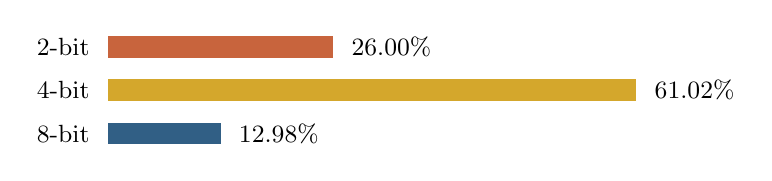
\begin{tikzpicture}[x=0.11cm,y=0.55cm]
  \node[anchor=east,font=\small] at (0,2) {2-bit};
  \fill[taqclay] (1,1.75) rectangle (27,2.25);
  \node[anchor=west,font=\small] at (28,2) {26.00\%};
  \node[anchor=east,font=\small] at (0,1) {4-bit};
  \fill[taqgold] (1,0.75) rectangle (62,1.25);
  \node[anchor=west,font=\small] at (63,1) {61.02\%};
  \node[anchor=east,font=\small] at (0,0) {8-bit};
  \fill[taqblue] (1,-0.25) rectangle (14,0.25);
  \node[anchor=west,font=\small] at (15,0) {12.98\%};
\end{tikzpicture}
}
\caption{Parameter mass distribution of the selected 2/4/8-bit policy.}
\label{fig:policy-mass}
\end{figure}

\section{Results}

\subsection{MMLU-coding}

Table~\ref{tab:mmlu} reports the current MMLU-coding last100 results. BF16 and INT8 are strong. Uniform INT4 reaches 91\%, and the mixed policy also reaches 91\%. This benchmark therefore does not currently establish a mixed-over-INT4 win. It does, however, show that the exact-budget policy remains competitive with INT4 while changing a large fraction of groups.

\begin{table}[t]
\caption{MMLU-coding last100 results. Prompt style is simple-evals; max new tokens is 4096.}
\label{tab:mmlu}
\centering
\footnotesize
\begin{tabular}{lrrrr}
\toprule
Model & Correct & Acc. & Cap & Lat. \\
\midrule
BF16 & 95/100 & 95\% & 0 & 9.14s \\
Uniform INT8 & 94/100 & 94\% & 2 & 46.21s \\
Uniform INT4 & 91/100 & 91\% & 5 & 66.88s \\
Mixed 2/4/8 & 91/100 & 91\% & 3 & 12.29s \\
\bottomrule
\end{tabular}
\end{table}

\subsection{MATH-500}

Table~\ref{tab:math500} reports MATH-500 last100 results for a separate MATH-oriented exact-budget policy. This policy is not the same artifact as the coding policy used for HumanEval and BigCodeBench; it comes from the earlier exact-budget frontier with hash \texttt{9bbaf3a...59b9e9}. The MATH policy improves over uniform INT4 from 80\% to 84\%, while BF16 reaches 86\%. It also reduces length-capped examples from 14 to 7 and has lower mean latency than both BF16 and uniform INT4 in this run.

\begin{table}[t]
\caption{MATH-500 last100 results. Prompt style is simple-evals non-thinking; max new tokens is 4096.}
\label{tab:math500}
\centering
\footnotesize
\begin{tabular}{lrrrr}
\toprule
Model & Correct & Acc. & Cap & Lat. \\
\midrule
BF16 & 86/100 & 86\% & 7 & 50.58s \\
Uniform INT4 & 80/100 & 80\% & 14 & 71.27s \\
MATH mixed & 84/100 & 84\% & 7 & 36.78s \\
\bottomrule
\end{tabular}
\end{table}

\subsection{HumanEval and EvalPlus}

HumanEval/EvalPlus gives the clearest positive signal for the current policy. Uniform INT4 loses 6.7 points relative to INT8 on HumanEval base and 5.5 points on HumanEval+. The mixed policy recovers 3.7 points on HumanEval base and 3.0 points on HumanEval+ while staying at the INT4-sized raw footprint. It does not match INT8, but it narrows the INT4 gap.

\begin{table}[t]
\caption{Official EvalPlus results with greedy generation and max new tokens 768.}
\label{tab:evalplus}
\centering
\begin{tabular}{lrr}
\toprule
Model & HumanEval base & HumanEval+ \\
\midrule
BF16 & 87.8\% & 82.3\% \\
Uniform INT8 & 89.0\% & 82.3\% \\
Uniform INT4 & 81.1\% & 76.8\% \\
Mixed 2/4/8 & 84.8\% & 79.9\% \\
\bottomrule
\end{tabular}
\end{table}

\begin{figure}[t]
\centering
\resizebox{0.95\columnwidth}{!}{%
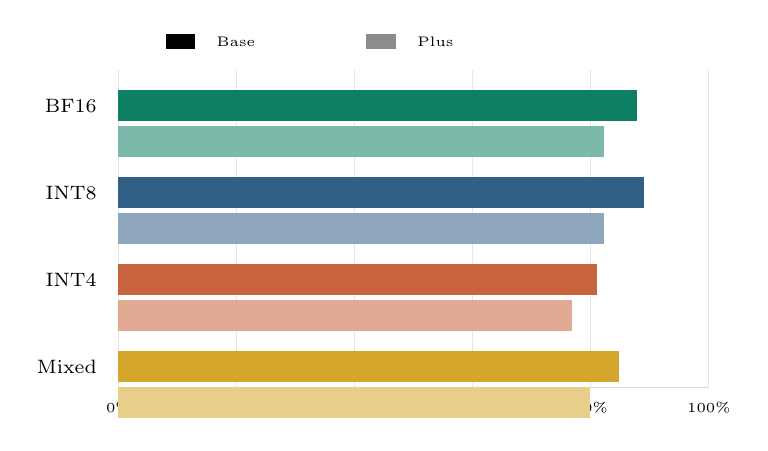
\begin{tikzpicture}[x=0.075cm,y=0.065cm]
  \draw[black!15] (0,0) -- (100,0);
  \foreach \x in {0,20,40,60,80,100} {
    \draw[black!10] (\x,0) -- (\x,62);
    \node[font=\tiny] at (\x,-4) {\x\%};
  }
  \node[anchor=east,font=\scriptsize] at (-2,55) {BF16};
  \fill[taqgreen] (0,52) rectangle (87.8,58);
  \fill[taqgreen!55] (0,45) rectangle (82.3,51);
  \node[anchor=east,font=\scriptsize] at (-2,38) {INT8};
  \fill[taqblue] (0,35) rectangle (89.0,41);
  \fill[taqblue!55] (0,28) rectangle (82.3,34);
  \node[anchor=east,font=\scriptsize] at (-2,21) {INT4};
  \fill[taqclay] (0,18) rectangle (81.1,24);
  \fill[taqclay!55] (0,11) rectangle (76.8,17);
  \node[anchor=east,font=\scriptsize] at (-2,4) {Mixed};
  \fill[taqgold] (0,1) rectangle (84.8,7);
  \fill[taqgold!55] (0,-6) rectangle (79.9,0);
  \fill[black] (8,66) rectangle (13,69);
  \node[anchor=west,font=\tiny] at (15,67.5) {Base};
  \fill[black!45] (42,66) rectangle (47,69);
  \node[anchor=west,font=\tiny] at (49,67.5) {Plus};
\end{tikzpicture}
}
\caption{HumanEval/EvalPlus pass@1. Mixed recovers part of the uniform INT4 degradation.}
\label{fig:evalplus}
\end{figure}

\subsection{BigCodeBench-Hard}

BigCodeBench-Hard is the most realistic code benchmark in the current suite because it is generative, dependency-heavy, and closer to practical code synthesis than multiple-choice coding questions. We use the official BigCodeBench instruct prompt builder, not a simple-evals multiple-choice prompt. The runner writes generation artifacts to persistent storage and then runs execution grading on those saved samples, so grading can be retried without regenerating completions.

Table~\ref{tab:bigcodebench} reports the completed BigCodeBench-Hard results. Uniform INT4 drops sharply from BF16, reaching only 25/148 passing tasks. The mixed policy reaches 35/148, recovering 10 passing tasks over uniform INT4 while using the same raw INT4-sized footprint. It remains below INT8 and BF16, so the result supports a recovery claim rather than a quality-ceiling claim.

\begin{table}[t]
\caption{BigCodeBench-Hard execution results. Generation uses the official instruct prompt with max new tokens 1280; grading uses pass@1.}
\label{tab:bigcodebench}
\centering
\footnotesize
\begin{tabular}{lrrrr}
\toprule
Model & Correct & Pass@1 & Cap & Avg tok. \\
\midrule
BF16 & 43/148 & 29.05\% & 2 & 512.2 \\
Uniform INT8 & 40/148 & 27.03\% & 2 & 511.0 \\
Uniform INT4 & 25/148 & 16.89\% & 2 & 533.7 \\
Mixed 2/4/8 & 35/148 & 23.65\% & 4 & 501.7 \\
\bottomrule
\end{tabular}
\end{table}

The token statistics are also informative. Mixed uses fewer average completion tokens than uniform INT4 (501.7 vs. 533.7) and a lower p95 completion length (872.6 vs. 933.7), but it has two additional capped examples. This means the mixed policy is not simply spending more tokens to pass more tests; its improvement over INT4 appears in spite of shorter average completions.

\section{Discussion}

The results support a careful interpretation. The current policy is not a universal improvement over all baselines. INT8 remains close to BF16 and is difficult to beat in quality. MMLU-coding does not separate mixed from uniform INT4. However, HumanEval/EvalPlus, BigCodeBench-Hard, and the MATH-oriented MATH-500 run show that exact-budget mixed policies can recover a meaningful portion of the INT4 degradation under the same raw weight footprint. This is exactly the type of signal that motivates task-aware mixed precision.

The most important systems result is that the new route is controllable. The policy has a clear budget, clear group assignments, and a stable construction process. This matters because MPQ experiments are expensive: each candidate may require PTQ, artifact validation, and benchmark evaluation. A reproducible search coordinate is more valuable at this stage than a broad stochastic search that is hard to debug.

\paragraph{Why generative benchmarks separate more clearly.}
MMLU-coding is multiple-choice. It may not stress long-form code synthesis in the same way as HumanEval or BigCodeBench. The coding policy was selected using MMLU-coding sensitivity, but the final signal appears stronger on generative code. The MATH-500 result adds a complementary example: when the frontier is built for a math workload, mixed precision recovers much of the uniform INT4 loss on math. This suggests that benchmark format and profiler alignment both matter.

\paragraph{Latency observations.}
The current MMLU-coding latency numbers should not be overinterpreted because backend kernels and artifact formats differ across quantized models. Mixed appears much faster than uniform INT4 on this particular run, but raw weight footprint is the budget we controlled, not end-to-end serving cost. A complete systems evaluation should report peak VRAM, decode tokens/sec, prefill latency, and kernel dispatch overhead.

\paragraph{What the present evidence can and cannot claim.}
The strongest current claim is not that mixed precision has already beaten every baseline. It has not. The defensible claim is narrower: after replacing the unstable evolutionary route with a structured exact-budget route, we obtained a real INT4-sized mixed artifact that matches INT4 on MMLU-coding and improves over INT4 on generative code evaluation. BigCodeBench-Hard now confirms the HumanEval trend on a larger and more realistic benchmark: mixed passes 35 tasks while uniform INT4 passes 25. That is a useful systems result because it converts the project from a noisy search story into a reproducible policy-construction story.

\paragraph{Interpretation of INT8.}
Uniform INT8 is not treated as a same-budget baseline. It is a quality ceiling and sanity check. In the current results, INT8 is close to BF16 on both MMLU-coding and HumanEval/EvalPlus. This is expected for a strong 9B model and modern PTQ tooling. The mixed policy is not trying to beat INT8 at the same footprint; it is trying to recover as much of the INT8/BF16 quality as possible while staying near the raw footprint of INT4.

\section{Ablation Plan}

Several ablations follow directly from the current route. First, the sensitivity profiler should be rerun on the same prompt protocol as the final benchmark. Early experiments showed that prompt choice can shift absolute accuracy substantially, so policy construction should not rely on a profiling prompt that differs from evaluation. Second, the frontier coordinate should be swept more densely around \policyid{}. The current policy comes from a coarse-to-fine path, but a local neighborhood around path index 112 can still contain policies with better allocation at the same raw footprint. Third, the demotion side should be stress-tested: if too many high-mass MLP groups are moved to 2-bit, generation quality may fail on tasks that require long dependency chains even if multiple-choice accuracy remains stable.

The most important baseline ablation is a random exact-budget policy family. A small set of random 2/4/8 policies repaired to the same raw footprint would show whether the structured frontier is genuinely doing useful allocation or merely benefiting from the availability of some 8-bit groups. A second useful baseline is a TAQ-style fixed-ratio policy, for example assigning a fixed fraction of groups to 8-bit and the rest to 4-bit or 2-bit according to size constraints. These baselines would make the story stronger because they compare against simpler mixed-precision recipes, not only against uniform INT4.

\begin{table}[t]
\caption{Claim boundary for the current snapshot. ``Supported'' means supported by completed results in this paper; ``open'' marks claims that still need additional validation.}
\label{tab:claims}
\centering
\footnotesize
\begin{tabular}{p{0.38\columnwidth}p{0.50\columnwidth}}
\toprule
Claim & Status \\
\midrule
Exact INT4-sized raw footprint & Supported by policy accounting \\
Real PTQ artifact, not surrogate only & Supported by quantized artifact path \\
Mixed $>$ INT4 on MMLU-coding & Not supported; both are 91\% \\
MATH mixed $>$ INT4 on MATH-500 & Supported in last100 run \\
Mixed $>$ INT4 on HumanEval/EvalPlus & Supported in current run \\
Mixed closes gap to INT8/BF16 & Partially supported across tasks \\
Broad task-aware superiority & Pending cross-task tests \\
\bottomrule
\end{tabular}
\end{table}

\section{Limitations}

This is an engineering snapshot, not a final paper-grade claim. The evaluation slices are small: MMLU-coding and MATH-500 last100 have 100 examples each, HumanEval has 164 tasks, and BigCodeBench-Hard has 148 tasks. The coding policy was selected using MMLU-coding, and the MATH policy is a separate exact-budget artifact, so stronger cross-task validation is needed before claiming broad task awareness. Finally, exact raw weight footprint does not imply exact runtime memory or throughput equivalence.

Another limitation is that the sensitivity signal itself may be improvable. The current policy has many 8-bit groups but only 12.98\% of parameter mass in 8-bit. This structure is reasonable, but it depends on the ranking quality. Since BigCodeBench shows mixed above INT4 but still below INT8, the next step should be improving the sensitivity profiler and candidate generator rather than returning immediately to unconstrained evolutionary search.

\paragraph{Statistical power.}
The completed evaluations are not yet large enough for strong statistical claims about small margins. A one- or two-point difference on 100 examples should be treated as inconclusive. The HumanEval/EvalPlus improvements are larger and use the full benchmark, but even there the task count is only 164. A final paper should report confidence intervals or paired tests wherever per-example outputs are available.

\paragraph{Deployment metrics.}
Raw footprint is the controlled budget, but production systems care about peak VRAM and throughput. Mixed precision may reduce weight bytes while increasing kernel complexity. Conversely, some artifact formats may run faster or slower for reasons that are independent of the bit allocation itself. A complete MLSys submission should therefore include hardware-normalized decode tokens/sec, prefill latency, peak memory, and possibly energy or cost per generated token.

\section{Next Steps}

The immediate next step is to rerun the profiler and candidate generator with the final prompt protocol, then repeat the coarse-to-fine frontier search around the current best region. The second step is to add random exact-budget and fixed-ratio mixed baselines. These additions would separate three possible explanations for the current generative-code signal: the frontier is genuinely task-aware, any mixed policy helps, or the observed gain is benchmark noise.

The method should be extended to a controlled cross-task test of task specificity. The expected evidence would be cross-task asymmetry: a policy selected for code should perform best on code, while a policy selected for math should recover more quality on math. Without this cross-task comparison, the phrase ``task-aware'' remains plausible but not fully demonstrated.

\section{Conclusion}

We presented the current \method{} mainline for task-aware mixed-precision quantization under an exact INT4-sized raw weight budget. The main change is methodological: abandon evolutionary crossover as the primary search mechanism and use a deterministic 2/4/8-bit frontier that explicitly couples 8-bit promotions with 2-bit demotions. The resulting Qwen3.5-9B mixed policies are reproducible, budget-aligned, and real. Empirically, the coding policy matches uniform INT4 on MMLU-coding and improves over uniform INT4 on HumanEval/EvalPlus and BigCodeBench-Hard; a separate MATH-oriented policy improves over uniform INT4 on MATH-500 last100. The current story is therefore not that mixed precision beats INT8, but that structured exact-budget mixed precision recovers a substantial portion of the INT4 quality loss while preserving the raw INT4 footprint.

\section*{Acknowledgements}

Omitted for anonymous review.

\bibliography{ta_mpq_mlsys_paper}
\bibliographystyle{mlsys2025}

\end{document}
